\section{Results}
\label{sec:results}

The results so far are data checks and runs of the extraction models, and none of them answers either question yet.
The checks used the full tables, and the larger model runs read companion text rather than the skill body that extraction uses, so they show kinds of errors rather than how often those errors occur.

\subsection{License labels and companion text}

After trimming, lowercasing, and filling blank labels, the repository table held 42 distinct license strings, among them MIT, Apache-2.0, GPL-3.0, and AGPL-3.0.
These strings describe the repository that hosts a skill, so they are a data check rather than an answer about the projects that publish taught tools.
We also classified the 3{,}486{,}179 non-blank companion texts, and Table~\ref{tab:companion-kinds} shows that almost all of them are free text or JSON objects.
Both kinds include scripts and configuration, so companion text is not skill prose, and extraction for the study stays on the skill body.

\begin{table}[!t]
  \centering
  \caption{Kinds of non-blank companion text}
  \label{tab:companion-kinds}
  \begin{tabular}{lrr}
    \toprule
    Kind        & Rows          & Share (\%) \\
    \midrule
    Free text   & 3{,}236{,}628 & 92.8       \\
    JSON object & 238{,}834     & 6.9        \\
    JSON array  & 10{,}523      & 0.3        \\
    Other JSON  & 194           & 0.0        \\
    \bottomrule
  \end{tabular}

  \smallskip
  \footnotesize Other JSON is a JSON value that is a string, a number, a boolean, or null.
\end{table}

\subsection{Label-only model run}

We applied the label-only model at a score cutoff of~$0.8$ to a seeded draw of 500 companion texts, each clipped to its first 384 characters.
Fig.~\ref{fig:label-only-top} shows every span found in at least two texts.
No bar comes near 500 because the cutoff drops every lower-scoring span, so many texts return no span at all.
The chart also shows why a human check is needed.
The skill filename is marked as a tool even though it names the document itself, and GitHub, which leads with nine files, can be the site inside an address, the place the skill is published, or an attribution link.
None of these labels has a measured error rate yet.

\begin{figure}[!t]
  \centering
  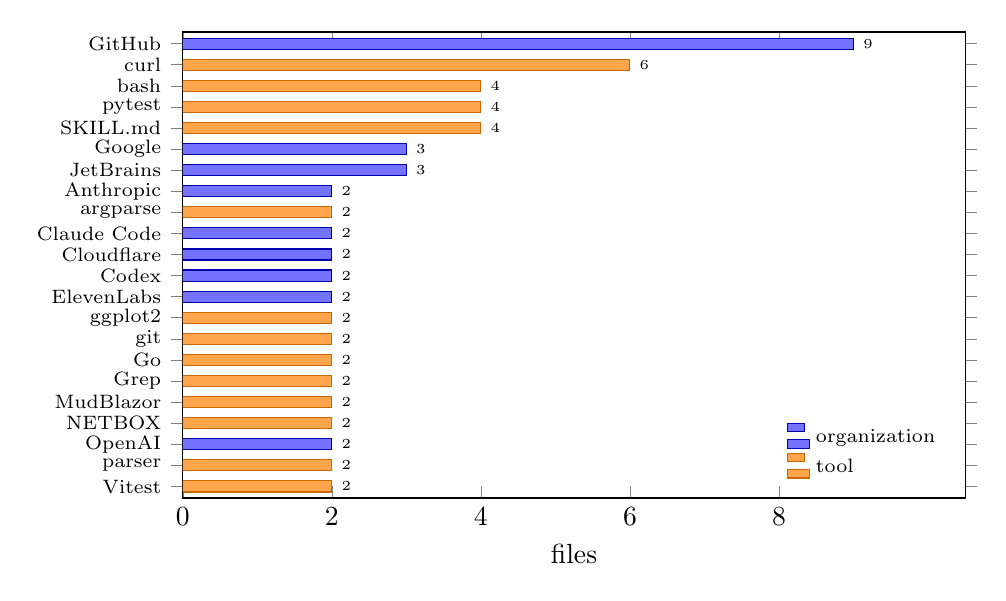
\begin{tikzpicture}
\begin{axis}[
  xbar,
  width=0.95\columnwidth,
  height=7.5cm,
  bar width=4pt,
  bar shift=0pt,
  enlarge y limits={abs=0.55},
  xmin=0,
  xmax=10.5,
  xtick={0,2,4,6,8},
  xlabel={files},
  ylabel={},
  ytick={1,...,22},
  yticklabels={
    Vitest,
    parser,
    OpenAI,
    NETBOX,
    MudBlazor,
    Grep,
    Go,
    git,
    ggplot2,
    ElevenLabs,
    Codex,
    Cloudflare,
    Claude Code,
    argparse,
    Anthropic,
    JetBrains,
    Google,
    SKILL.md,
    pytest,
    bash,
    curl,
    GitHub
  },
  yticklabel style={font=\scriptsize, anchor=east},
  nodes near coords,
  every node near coord/.append style={font=\tiny},
  nodes near coords align={horizontal},
  legend style={
    at={(0.98,0.02)},
    anchor=south east,
    font=\scriptsize,
    cells={anchor=west},
    draw=none,
    fill=none
  },
  legend cell align=left,
]
% y=22 is GitHub at the top of the chart.
\addplot[fill=blue!55, draw=blue!70!black] coordinates {
  (9,22)
  (3,17)
  (3,16)
  (2,15)
  (2,13)
  (2,12)
  (2,11)
  (2,10)
  (2,3)
};
\addplot[fill=orange!70, draw=orange!80!black] coordinates {
  (6,21)
  (4,20)
  (4,19)
  (4,18)
  (2,14)
  (2,9)
  (2,8)
  (2,7)
  (2,6)
  (2,5)
  (2,4)
  (2,2)
  (2,1)
};
\legend{organization,tool}
\end{axis}
\end{tikzpicture}

  \caption{Spans that the label-only model found in at least two of 500 companion texts at a score cutoff of 0.8, counted as distinct files after folding case.
    Bars stay small because many texts return no span above the cutoff.}
  \label{fig:label-only-top}
\end{figure}

\subsection{Relation model trials}

To try the organization link proposed in Section~\ref{sec:relation}, we ran a relation model, GLiNER Relex large, version~0.5,\footnote{Model card at \url{https://huggingface.co/knowledgator/gliner-relex-large-v0.5}.} on the same 500 companion texts at a cutoff of~$0.6$.
It linked a tunnel setting to Cloudflare as we would want, but it also tied \textit{python3} to a nearby word and a copied repository address to GitHub.
A trial on twelve short skill texts, drawn with its own fixed seed and with a length limit that applies only to that trial, still links the wrong pairs.
We read those rows manually, so they show where extraction fails but not how often.

Taken together, these results support keeping extraction on the skill body, and they show that label-only extraction at this cutoff counts names that are not taught tools.
They do not yet support any claim about tool frequency or licenses, which needs the validation sample and a run over the full population.
